\documentclass{article}
\usepackage{amsmath}
\usepackage{amssymb}
\usepackage{hyperref} % For clickable table of contents
\usepackage{tikz}
\usetikzlibrary{arrows.meta, positioning}

\title{CPSC 354 Report}
\author{Drew Floyd}
\date{}

\begin{document}

\maketitle
\tableofcontents
\newpage

\section{The MU-Puzzle}

MI $\rightarrow$ MU

\textbf{Rule 1:} If you possess a string whose last letter is \texttt{I}, add \texttt{U}.

\textbf{Rule 2:} Suppose you have \texttt{Mx}, you may add \texttt{Mxx}.

\textbf{Rule 3:} If \texttt{III} occurs in one of the strings, you may make a new string with \texttt{U} in place of \texttt{III}.

\textbf{Rule 4:} If \texttt{UU}, you can drop it.

\vspace{1em}

MI \\
MII $\; Mxx$ \\
MIIII $\; Mxx$ \\
MIIIIIIII $\; Mxx$ \\
MUIIU $\; MIU$ \\
$\varnothing$

\vspace{1em}

MI $\; \rightarrow$ use $Mxx$ rule $\infty$ times \\
MIIII... \\

No matter what Rule you use you will never be able to get 0 Mod3, because I will always be 1 mod 3 or 2 mod 3

\vspace{1em}

\texttt{MUUU} \\
\texttt{MIII}

\vspace{1em}

\textbf{Rule 1} does not affect \# of I's. \\
\textbf{Rule 2} does not give 0 mod 3. \\
\textbf{Rule 3} does not solve the problem as removing 3 I's does not change the output of mod3. \\
\textbf{Rule 4} does not change the \# of I's. \\

We can never get rid of all of the I's, 0 mod 3 is not possible. Thus you cannot get MU from MI.

\newpage

\section{Rewriting Assignment}

\begin{enumerate}
    \item $A = \{ \}$ \\
    \hspace*{1em} $R = \{ \}$
% #1
    \begin{center}
        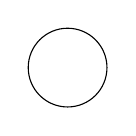
\begin{tikzpicture}
        \node[circle, draw, minimum size=1cm] (a) {};
        % Ensure the node is properly placed and visible
        \path (a) ++(0,0);
        \end{tikzpicture}
        \end{center}
    This diagram is terminating because there are no infinite loops, confluent because all paths lead to the same result, and has a unique normal form as there is only one final state.

\vspace{4em}

    \item $A = \{ a \}$ \\
    \hspace*{1em} $R = \{ \}$
% #2
    \begin{center}
    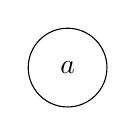
\begin{tikzpicture}
        \node[circle, draw, minimum size=1cm] (a) {$a$};
    \end{tikzpicture}
    \end{center}
    This diagram is terminating because there are no infinite loops, confluent because all paths lead to the same result, and has a unique normal form as there is only one final state.

\vspace{4em}

    \item $A = \{ a \}$ \\
    \hspace*{1em} $R = \{ (a,a) \}$
% #3
    \begin{center}
    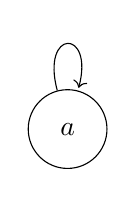
\begin{tikzpicture}
        \node[circle, draw, minimum size=1cm] (a) {$a$};
        \draw[->] (a) edge[loop above] (a);
    \end{tikzpicture}
    \end{center}
    This diagram is not terminating due to the presence of infinite loops, confluent because all paths merge, but does not have a unique normal form as multiple results are possible.

\vspace{6em}

    \item $A = \{ a, b, c \}$ \\
    \hspace*{1em} $R = \{ (a,b), (a,b) \}$
% #4
    \begin{center}
    \begin{tikzpicture}
        \node[circle, draw, minimum size=1cm] (a) {$a$};
        \node[right=2cm of a, circle, draw, minimum size=1cm] (b) {$b$};
        \node[below=2cm of a, circle, draw, minimum size=1cm] (c) {$c$};
        \draw[->] (a) -- (b);
        \draw[->] (a) -- (c);
    \end{tikzpicture}
    \end{center}
    This diagram is terminating as there are no infinite loops, not confluent because paths diverge, and does not have a unique normal form due to multiple end states.

\vspace{4em}

    \item $A = \{ a, b \}$ \\
    \hspace*{1em} $R = \{ (a,a), (a,b) \}$
%  #5
    \begin{center}
    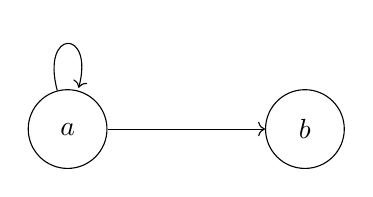
\begin{tikzpicture}
        \node[circle, draw, minimum size=1cm] (a) {$a$};
        \node[right=2cm of a, circle, draw, minimum size=1cm] (b) {$b$};
        \draw[->] (a) -- (b);
        \draw[->] (a) edge[loop above] (a);
    \end{tikzpicture}
    \end{center}
    This diagram is not terminating due to the presence of infinite loops, confluent because all paths lead to b, it has a unique normal form as the single end state is b.

\vspace{4em}

    \item $A = \{ a, b, c \}$ \\
    \hspace*{1em} $R = \{ (a,b), (b,b), (a,c) \}$
%  #6
    \begin{center}
    \begin{tikzpicture}
        \node[circle, draw, minimum size=1cm] (a) {$a$};
        \node[right=2cm of a, circle, draw, minimum size=1cm] (b) {$b$};
        \node[below=2cm of a, circle, draw, minimum size=1cm] (c) {$c$};
        \draw[->] (a) -- (b);
        \draw[->] (a) -- (c);
        \draw[->] (b) edge[loop above] (b);
    \end{tikzpicture}
    \end{center}
    This diagram is not terminating due to the presence of infinite loops, not confluent because paths diverge, and has a unique normal form due to having a single end state on c.

\vspace{4em}

    \item $A = \{ a, b, c \}$ \\
    \hspace*{1em} $R = \{ (a,b), (b,b), (a,c), (c,c) \}$
% #7
    \begin{center}
    \begin{tikzpicture}
        \node[circle, draw, minimum size=1cm] (a) {$a$};
        \node[right=2cm of a, circle, draw, minimum size=1cm] (b) {$b$};
        \node[below=2cm of a, circle, draw, minimum size=1cm] (c) {$c$};
        \draw[->] (b) edge[loop above] (b);
        \draw[->] (c) edge[loop below] (c);
        \draw[->] (a) -- (b);
        \draw[->] (a) -- (c);
    \end{tikzpicture}
    \end{center}
    This diagram is not terminating due to the presence of infinite loops, not confluent because paths diverge, and does not have a unique normal form due to no end states.

\vspace{4em}

\end{enumerate}

\section*{Properties}
\begin{tabular}{c c c c p{8cm}}
     T & C & U & Example(s) & Explanation \\ \hline
    True & True & True & 1, 2 & These examples terminate, are confluent, and have a unique normal form because all paths lead to a single final state without divergence or loops. \\
    True & True & False & None & This state is impossible because confluence implies a unique normal form when termination is true. \\
    True & False & True & None & This state is impossible because non-confluence means paths diverge, which contradicts having a unique normal form. \\
    True & False & False & 4 & This example terminates but is not confluent due to diverging paths and does not have a unique normal form as multiple end states exist. \\
    False & True & True & 5 & This example does not terminate because a is a loop, but since it loops on itself it can still be confluent and point to b to result in a unique normal form. \\
    False & True & False & 3 & This example does not terminate but is confluent because all paths merge, though it does not have a unique normal form due to multiple results. \\
    False & False & True & None & This state is impossible because non-termination and non-confluence contradict having a unique normal form. \\
    False & False & False &  6, 7 & These examples do not terminate, are not confluent due to diverging paths, and do not have a unique normal form as no single end state exists. \\
\end{tabular}

\vspace{4em}
\noindent T: Terminating, C: Confluent, U: Unique Normal Form

\end{document}
